\definecolor{Gray}{gray}{0.85}
\definecolor{LightCyan}{rgb}{0.88,1,1}
  \renewcommand{\theequation}{\arabic{chapter}.\arabic{equation}}
\newcolumntype{a}{>{\columncolor{Gray}}c}
	\chapter{LANDASAN TEORI}
	Bab ini akan membahas mengenai dasar teori dan literatur yang menjadi dasar pengerjaan tugas akhir ini. Pada subbab 2.1 membahas mengenai definisi umum yang digunakan dalam memecahkan permasalahan ini. Pada subbab 2.2 membahas mengenai deskripsi permasalahan. Pada subbab 2.3 membahas mengenai contoh permasalahan. Pada subbab 2.4 membahas mengenai penyelesaian masalah secara lengkap.
	\section{Definisi Umum}
	Pada subbab ini membahas definisi-definisi yang digunakan sebagai dasar untuk memahami permasalahan ini dan pemecahannya.	
	\subsection{Polyalphabetic Cipher}
	\textit{Polyalphabetic Cipher }merupakan salah satu teknik untuk menenkripsi dengan menggunakan subtitusi huruf untuk menyubtitusikannya. Secara garis besar yang dimaksud dengan \textit{polyalphabetic cipher} memiliki 2 aturan dasar yang harus dipenuhi yaitu :
	\begin{enumerate}
		\item Memiliki satu set aturan subtitusi \textit{monoalphabetic cipher} yang digunakan.
		\item Sebuah kunci mengatur suatu aturan tertentu yang dipilih untuk mengatur transformasi yang dilakukan.
	\end{enumerate}
	Untuk memperjelas aturan di atas, dapat dilihat pada Gambar \ref{fig:polyalphabeticalcipher}.
	\begin{figure}[H]
		\centering
		%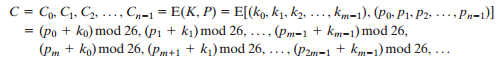
\includegraphics[scale=0.85]{images/bab2/poly.png}
		\begin{align*}
 		C &=c_0,c_1,c_2,...,c_{n-1} \\
      	E(K,P)&=E[(k_0,k_1,...,k_{m-1})(p_0,p_1,...,p_{n-1})] \\
      	&=(p_0+k_0)mod26,(p_1+k_1)mod26,...,(p_{m-1}+k_{m-1})mod26, \\
      		&(p_m+k_0)mod26,(p_{m+1}+k_1)mod26,...,(p_{2m-1}+k_{m-1})mod26,...
		\end{align*}		
		
		\caption{Aturan \textit{Polyalphabetical Cipher}}
		\label{fig:polyalphabeticalcipher}
	\end{figure}
	Di mana $C$ adalah \textit{ciphertext}, $E$ adalah fungsi enskripsi, $K$ adalah kunci, dan $P$ adalah \textit{plaintext}.
	Salah satu turunan dari \textit{polyalphabetic cipher} adalah teknik \textit{Vigenere Cipher} yang menjadi dasar permasalahan yang diangkat dalam tugas akhir ini\cite{stallings_computer_2015}.
	
	\subsection{Ciphertext}
	\textit{Ciphertext} adalah suatu pesan / teks acak yang dihasilkan dari suatu algoritma kriptografi. 
	Contoh dari \ciphertext dalam kasus \textit{polyalphabetical cipher} adalah "RTPPRKGFI" yang merupakan hasil enkripsi dari "PLAINTEXT" dan menggunakan kunci "CIPHER"\cite{william_crytography_2011}.
	
	\subsection{Plaintext}
	\textit{Plaintext} adalah data original sebagai inputan dari suatu metode enskripsi yang akan dilakukan\cite{william_crytography_2011}. Biasanya merupakan suatu rangkaian kata yang masih dapat dipahami artinya atau hasil keluaran dari suatu algoritma kriptografi yang akan dienskripsi lagi.
	
	\subsection{Secret Key}
	\textit{Secret Key} atau yang lebih dikenal dengan \textit{key} adalah suatu inputan dari algoritma enskripsi yang akan menentukan suatu transformasi dan subtitusi yang akan dilakukan oleh algoritma enskripsi\cite{william_crytography_2011}. Dalam kasus \textit{polyalphabetical cipher} pada permasalahan yang diangkat dalam tugas akhir ini, panjang kunci yang digunakan setidaknya 1. 
	
	\subsection{Friedman test}
	\textit{Friedman test} atau \textit{Kappa Test} merupakan salah satu metode yang digunakan untuk mendeskripsikan \textit{Polyalphabetical Cipher} dengan menggunakan \textit{index of coincidence}. \textit{Index of coincidence} digunakan untuk mengukur tingkat ketidakrataan frekuensi \textit{ciphertext}. Untuk menghitung \textit{index of coincidence} digunakan persamaan \ref{eq:12}\cite{henk_encyclopedia_2005}.
	\begin{equation} \label{eq:12}
	\begin{split}
	IC&=c*((\frac{n_a}{N}*\frac{n_a-1}{N-1})+(\frac{n_b}{N}*\frac{n_b-1}{N-1})+ \\
	&(\frac{n_c}{N}*\frac{n_c-1}{N-1})+...+(\frac{n_z}{N}*\frac{n_z-1}{N-1}))\\
	\end{split}
	\end{equation}
	Persamaan \ref{eq:12} dapat disederhanakan menjadi persamaan \ref{eq:13}.
	\begin{equation} \label{eq:13}
	IC=\frac{\sum_{i=1}^{c}n_i(n_i-1)}{\frac{N*(N-1)}{c}}
	\end{equation}
	$IC$ adalah \textit{index of coincidence}, $n_a$ adalah jumlah huruf "a" yang terdapat pada suatu \textit{ciphertext} dan seterusnya, $N$ adalah jumlah huruf yang terdapat pada \textit{ciphertext}, $c$ adalah jumlah huruf dalam alfabet. Karena tidak dapat mengetahui jumlah huruf yang mungkin terbentuk dalam alfabet yang ada dan harus mengetahui jumlah setiap huruf yang muncul dalam suatu \textit{ciphertext}. Karena keterbatasan informasi mengenai \ciphertext yang didapatkan, maka metode ini tidak dapat digunakan untuk menyelesaikan permasalahan dalam tugas akhir ini.
	
	 \subsection{Kasiski Examination}
	 \textit{Kasiski Examination} merupakan suatu teknik yang digunakan untuk mendeskripsikan secara paksa suatu \textit{ciphertext} yang menggunakan teknik substitusi, baik itu \textit{polyalphabetical cipher} maupun \textit{monoalphabetical cipher}. Teknik menggunakan kelemahan yang ditimbulkan oleh teknik substitusi itu sendiri. Yaitu apabila suatu \textit{subtring} dari \plaintext dan \textit{subtring} dari suatu set kunci yang berulang terdapat yang berulang, maka dapat dipastikan untuk menebak panjang huruf / karakter kunci yang digunakan, tanpa diketahui \plaintext dan kuncinya. Sebagai contoh dapat dilihat pada Tabel \ref{tab:kasiskiexamination}.
	 \begin{table}[H]
	 	\caption{Contoh \textit{Kasiski Examintaion}}
		\resizebox{\textwidth}{!}{%
		\begin{tabular}   {|c|c|c|c|c|c|c|c|c|c|c|c|c|c|c|c|}\hline
		\textit{ciphertext}&C&S&A&S&X&S&J&O&S&P&C&S&A&S&X \\ \hline
		%kunci              &a&b&c&d&e&a&b&c&d&e&a&b&c&d&e \\ \hline
		\end{tabular}}
		\label{tab:kasiskiexamination}
	\end{table}
	Dari Tabel \ref{tab:kasiskiexamination} yang ada dapat disimpulkan bahwa kata "CSASX" berulang. Sehingga setidaknya dapat disimpulkan bahwa panjang kuncinya mungkin 5 karakter atau faktor dari 10\cite{noauthor_kasiski_nodate}.
	Cara pencarian panjangnya:
	\begin{enumerate}
	\item Mencari semua subtring yang berulang. Seperti Tabel \ref{tab:kasiskiexamination}.
	\item Mencari semua faktor kapan subtring itu berulang lagi sebagai contoh Tabel \ref{tab:kasiskiexamination} itu selisih antara sub kalimat "CSASX" adalah 10. Maka, faktor dari 10 adalah 10,5,2,1. 
	\item Kemungkinan besar faktor yang sering berulang adalah jawabannya. 
	\end{enumerate}
	 Hal ini yang menjadi dasar pengerjaan permasalahan yang diangkat dalam tugas akhir ini.
 
	\subsection{Intersection}
	\textit{Intersection} adalah himpunan A dan himpunan B di mana ada bagian dari A juga merupakan bagian dari B. Sehingga dapat ditulis dengan persamaan \ref{eq:intersect}.
	\begin{equation}
	\label{eq:intersect}
	A\cap{B=\{x:x\in A \textrm{ dan } x \in B \}}
	\end{equation}
	Sebagai contoh \textit{intersection} antara $\{1,2,3\}$ dan $\{1,4,5\}$ adalah $\{1\}$\cite{devlin_joy_1993}	.
	
	\section{Deskripsi Permasalahan}
	\label{chapter:dasar-teori}
	Permasalahan yang diangkat dalam tugas akhir ini diangkat dari suatu permasalahan yang terdapat pada suatu situs penilaian daring atau \textit{online judge} SPOJ yaitu \textit{The Bytelandian Cryptographer (Act IV)} dengan nomer soal 20 dengan kode soal CRYPTO4. Deskripsi soal yang asli menggunakan bahasa Inggris dapat dilihat pada Gambar \ref{fig:crypto4_def}\cite{piwakowski_crypto4_2004}.
	
	
	 Permasalahan pada The Bytelandian Cryptographer (Act IV) diberikan pesan dengan panjang $N$ huruf, huruf yang digunakan adalah huruf kapital latin dari A sampai dengan Z, yang dapat ditafsirkan menjadi bilangan bulat dari 0 sampai dengan 25. Diberikan kunci untuk mentransmisikan pesan yang diketahui oleh kedua belah pihak yang terdiri dari $M$ bilangan bulat. Dengan menggunakan kunci yang ada bahwa pada index ke $i$ dari pesan pada index $x_i$ akan di enkripsikan ke dalam bentuk index ke $i$ dari pesan hasil enskripsi $y$, yang mengikuti aturan \ref{eq:hahah}.
	\begin{equation}
	y_i=x_i+k_{1+(i-1)mod M} mod 26 
	\label{eq:hahah}
	\end{equation}		 
	 Diketahui \textit{plaintext} dan \textit{ciphertext} yang diberikan hanya berupa potongan-potongan dari kedua pesan tersebut. Dicari bagaimana menkonstruksi ulang pesan yang telah didapat sehingga bisa membentuk \textit{plaintext} yang asli dari pesan yang telah didapatkan sebanyak-banyaknya.
	\begin{figure}[H]
		\centering
		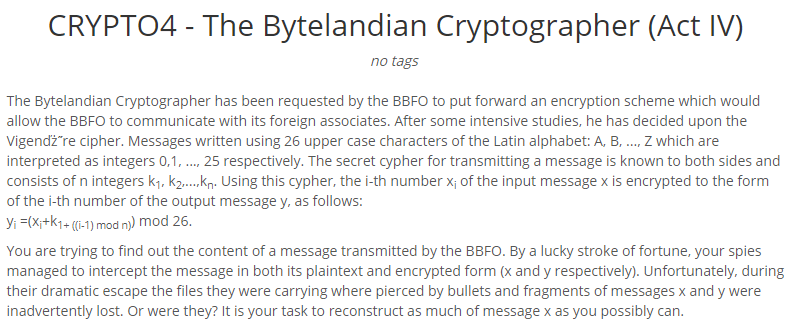
\includegraphics[scale=0.75]{images/bab2/crypto_def.png}
		\caption{Deskripsi Permasalahan dalam Bahasa Inggris pada SPOJ \textit{The Bytelandian Cryptographer (Act IV)}}
		\label{fig:crypto4_def}
	\end{figure}
	
	Deskripsi mengenai format masukan sebagai berikut:
	\begin{enumerate}
	\item Baris pertama berisi sejumalah $T$ kasus uji coba
	\item Setiap kasus uji coba, baris pertama berisi $1$ bilangan bulat $M$ dimana merupakan sejumlah batas atas panjang kunci yang digunakan 
	\item Baris kedua dari setiap kasus uji coba berisi \textit{plaintext}.
	\item Baris ketiga dari setiap kasus uji coba berisi \textit{ciphertext}.
	%\item \textit{Plaintext} dan \textit{ciphertext} direpresentasikan dengan karakter 'A' sampai dengan 'Z'.
	\end{enumerate}
	\textit{Plain text} dan \textit{ciphertext} dalam format masukan menggunakan karakter A sampai dengan Z yang dapat ditafsirkan kedalam bilangan bulat 0 sampai dengan 25 dan karakter '*' yang dapat ditafsirkan sebagai karakter yang hilang.
	
	
	Format keluaran yang dihasilkan adalah 1 baris \textit{plaintext} yang dapat direkontruksi dan '*' apabila nilai dari karakter pada posisi tersebut tidak dapat ditentukan. 
	Batasan permasalahan \textit{The Bytelandian Cryptographer (Act IV)} adalah sebagai berikut:
	\begin{enumerate}
		\item $T \leq 200$
		\item $1 \leq M \leq 100,000$
		\item Panjang \textit{input file} tidak melebihi dari 2MB.
		\item Lingkungan penilaian Intel Pentium G860 3GHz.
		\item Batas Waktu: $\leq17$ detik
		\item Batas Sumber Code : 50000B
		\item Batas Memory : 1536 MB.                 
	\end{enumerate}

	\section{Contoh Kasus Permasalahan}
	Dalam Permasalahan yang diangkat ini huruf A sampai dengan Z ditafsirkan sebagai 0 sampai dengan 25.
	Contoh 1. Diketahui $M$ bernilai 1 yang menunjukkan batas atas dari panjang kunci. Diketahui \plaintext adalah A*X*C dan \ciphertext adalah **CM*. 
	\begin{table}[H]
	 	\centering
		\caption{Contoh 1}	 	
	 	\begin{tabular}{|c|c|c|c|c|c|c|}\hline
	 	\textit{index}&0&1&2&3&4\\ \hline
	 	\textit{plain text}&A&*&X&*&C\\ \hline
	 	\textit{ciphertext}&*&*&C&M&*\\ \hline
	 	Selisih yang diketahui& & &5& & \\ \hline
	 	Hasil              &A&*&X&H&C\\ \hline
	 	\end{tabular}
	 	\label{tab:contoh1}
	\end{table}
	 
	 Dari Tabel \ref{tab:contoh1} dapat diketahui bagaimana hasil yang akan dicapai. Cara mencapai hasil yang diinginkan adalah sebagai berikut. Pertama-tama pencarian panjang kunci. Pada pencarian panjang kunci harus mengetahui dahulu batas atas dari panjang kunci tersebut. Pada contoh kasus ini $M$ bernilai 1, maka kemungkinan jawabannya hanya ada 1, yaitu $M$ itu sendiri, karena suatu panjang kunci yang digunakan dalam enskripsi tidak mungkin 0. Diasumsikan bahwa 1 warna mewakili satu blok kunci yang akan digunakan. Maka akan membentuk seperti pada Tabel \ref{tab:langkah1contoh1}.
	 
	\begin{table}[H]
	 	\centering
		\caption{Langkah 1 Contoh 1}	 	
	 	\setlength{\arrayrulewidth}{.08em}
	 	\begin{tabular}{|c|c|c|c|c|c|c|}\hline
	 	\textit{index}&0&1&2&3&4\\ \hline
	 	\textit{plain text}&\cellcolor{blue!15}A&\cellcolor{lime!15}*&\cellcolor{yellow!25}X&\cellcolor{green!15}*&\cellcolor{pink!25}C\\ \hline
	 	\textit{ciphertext}&\cellcolor{blue!15}*&\cellcolor{lime!15}*&\cellcolor{yellow!25}C&\cellcolor{green!15}M&\cellcolor{pink!25}*\\ \hline
	 	Selisih yang diketahui& & &5& & \\ \hline
	 	%Hasil              &A&*&X&H&C\\ \hline
	 	\end{tabular}
	 	\label{tab:langkah1contoh1}
	\end{table}
	
	  Karena selisih yang di ketahui hanya ada 1, maka itulah yang menjadi jawabannya. Selanjutnya mencari yang \plaintext yang bernilai "*" dan \ciphertext tidak kosong, seperti indeks ketiga. Maka indeks ketiga jawabannya adalah "H". Karena "M" $-$ $5$ adalah "H".
	 
	 
	 
	 Contoh 2. Diketahui bahwa $M$ bernilai 4 yang menunjukkan batas atas dari panjang kunci. Diketahui \plaintext adalah *B***A dan \ciphertext adalah AAAAAA. Dalam Contoh ini panjang kuncinya bisa dari 1 sampai dengan 4. 
	 \begin{table}[H]
	 	\centering
	 	\caption{Contoh 2}
	 	\begin{tabular}{|c|c|c|c|c|c|c|}\hline
		\textit{index}&0&1&2&3&4&5\\ \hline
	 	\textit{plain text}&*&B&*&*&*&A\\ \hline
	 	\textit{ciphertext}&A&A&A&A&A&A\\ \hline
	 	Selisih yang diketahui& &25& & & &0\\ \hline
	 	Panjang Kunci 1 & \multicolumn{6}{c|}{tidak bisa karena ada yang \textit{collision}}\\ \hline
	 	Panjang Kunci 2 & \multicolumn{6}{c|}{tidak bisa karena ada yang \textit{collision}}\\ \hline
	 	Panjang Kunci 3 &*&B&A&*&B&A \\ \hline
	 	Panjang Kunci 4 & \multicolumn{6}{c|}{tidak bisa karena ada yang \textit{collision}}\\ \hline
	 	\end{tabular}
	 	\label{tab:contoh2}
	\end{table}
	Cara yang harus dilalui adalah sebagai berikut. Pertama mencari panjang kunci yang bernilai diantara 1 - 4. \\
	Pada Tabel \ref{tab:k1contoh2} akan diperlihatkan proses pencarian ketika panjang kunci adalah 1.
	\begin{table}[H]
	 	\centering
	 	\caption{Panjang Kunci 1 Contoh 2}
	 	\setlength{\arrayrulewidth}{.08em}
	 	\begin{tabular}{|c|c|c|c|c|c|c|}\hline
		\textit{index}&0&1&2&3&4&5\\ \hline
	 	\textit{plain text}&\cellcolor{blue!15}*&\cellcolor{yellow!25}B&\cellcolor{green!15}*&\cellcolor{lime!25}*&\cellcolor{pink!30}*&\cellcolor{red!25}A\\ \hline
	 	\textit{ciphertext}&\cellcolor{blue!15}A&\cellcolor{yellow!25}A&\cellcolor{green!15}A&\cellcolor{lime!25}A&\cellcolor{pink!30}A&\cellcolor{red!25}A\\ \hline
	 	Selisih yang diketahui& &25& & & &0\\ \hline
	 	Panjang Kunci 1 & \multicolumn{6}{c|}{tidak bisa karena ada yang \textit{collision}}\\ \hline
	 	\end{tabular}
	 	\label{tab:k1contoh2}
	\end{table}	
	
	Apabila $1$ warna direpresentasikan menjadi 1 blok kunci, maka terdapat 5 blok kunci yang terbentuk. Pada bagian Tabel \ref{tab:k1contoh2} bahwa hanya ada 2 indeks di mana \plaintext dan \ciphertext yang diketahui. Kedua-duanya terletak pada blok kunci yang berbeda. Akan tetapi karena panjang bloknya $1$ maka tidak mungkin panjang kunci 1 dilakukan karena kedua-duanya saling bertabrakan dan membawa nilai yang berbeda. Yang menjadi permasalahan pada panjang kunci 1 adalah ketika blok yang diketahui bertabrakan dan masing masing membawa nilai yang berbeda juga. Sehinnga dapat disimpulkan bahwa panjang kunci 1 pada contoh kasus 2 tidak mungkin terjadi.
	\\
	Proses pencarian ketika panjang kunci adalah 2.
	\begin{table}[H]
	 	\centering
	 	\caption{Panjang Kunci 2 Contoh 2}
	 	\setlength{\arrayrulewidth}{.08em}
	 	\begin{tabular}{|c|c|c|c|c|c|c|}\hline
		\textit{index}&0&1&2&3&4&5\\ \hline
	 	\textit{plain text}&\cellcolor{blue!15}*&\cellcolor{blue!15}B&\cellcolor{green!15}*&\cellcolor{green!15}*&\cellcolor{pink!30}*&\cellcolor{pink!30}A\\ \hline
	 	\textit{ciphertext}&\cellcolor{blue!15}A&\cellcolor{blue!15}A&\cellcolor{green!15}A&\cellcolor{green!15}A&\cellcolor{pink!30}A&\cellcolor{pink!30}A\\ \hline
	 	Selisih yang diketahui& &25& & & &0\\ \hline
	 	Panjang Kunci 2 & \multicolumn{6}{c|}{tidak bisa karena ada yang \textit{collision}}\\ \hline
	 	\end{tabular}
	 	\label{tab:k2contoh2}
	\end{table}	
	
	Apabila 1 warna direprentasikan menjadi 1 blok kunci, maka terdapat 3 blok kunci yang terbentuk. Pada Tabel \ref{tab:k2contoh2} terlihat bahwa terdapat 2 indeks di mana \plaintext dan \ciphertext yang diketahui. Indeks yang pertama terletak pada blok pertama bagian akhir, begitu juga indeks yang kedua terletak pada blok 3 bagian akhir. Karena kedua-duanya terletak pada bagian akhir dari masing-masing blok maka dapat disimpulkan panjang kunci 2 juga tidak dapat digunakan.
	\\
	Proses Pencarian ketika panjang kunci adalah 3.
	\begin{table}[H]
	 	\centering
	 	\caption{Panjang Kunci 3 Contoh 2}
	 	\setlength{\arrayrulewidth}{.08em}
	 	\begin{tabular}{|c|c|c|c|c|c|c|}\hline
		\textit{index}&0&1&2&3&4&5\\ \hline
	 	\textit{plain text}&\cellcolor{blue!15}*&\cellcolor{blue!15}B&\cellcolor{blue!15}*&\cellcolor{green!15}*&\cellcolor{green!15}*&\cellcolor{green!15}A\\ \hline
	 	\textit{ciphertext}&\cellcolor{blue!15}A&\cellcolor{blue!15}A&\cellcolor{blue!15}A&\cellcolor{green!15}A&\cellcolor{green!15}A&\cellcolor{green!15}A\\ \hline
	 	Selisih yang diketahui& &25& & & &0\\ \hline
	 	Panjang Kunci 3 &*&B&A&*&B&A \\ \hline
	 	\end{tabular}
	 	\label{tab:k3contoh2}
	\end{table}	
	Apabila 1 warna direpresentasikan menjadi 1 blok kunci, maka terdapat 2 blok kunci yang terbentuk. Pada Tabel \ref{tab:k3contoh2} terlihat bahwa terdapat 2 indeks di mana \plaintext dan \ciphertext yang diketahui. Indeks yang pertama terletak dibagian tengah pada blok 1 dan indeks yang kedua terletak pada bagian akhir pada blok 2. Maka,  \plaintext yang terbentuk adalah pada bagian akhir dari blok kunci 1 dan bagian tengah dari blok kunci 2. Karena kedua-duanya saling melengkapi antara satu bagian dengan bagian lainnya. Sehingga hasil yang terbentuk pada bagian akhir dari blok kunci 1 adalah "A" $-$ $0$ adalah "A" dan bagian tengah dari blok kunci 2 adalah "A" $-$ $25$ adalah "B". 
	\\
	Proses pencarian ketika panjang kunci adalah 4
	\begin{table}[H]
	 	\centering
	 	\caption{Panjang Kunci 4 Contoh 2}
	 	\setlength{\arrayrulewidth}{.08em}
	 	\begin{tabular}{|c|c|c|c|c|c|c|}\hline
		\textit{index}&0&1&2&3&4&5\\ \hline
	 	\textit{plain text}&\cellcolor{blue!15}*&\cellcolor{blue!15}B&\cellcolor{blue!15}*&\cellcolor{blue!15}*&\cellcolor{green!15}*&\cellcolor{green!15}A\\ \hline
	 	\textit{ciphertext}&\cellcolor{blue!15}A&\cellcolor{blue!15}A&\cellcolor{blue!15}A&\cellcolor{blue!15}A&\cellcolor{green!15}A&\cellcolor{green!15}A\\ \hline
	 	Selisih yang diketahui& &25& & & &0\\ \hline
	 	Panjang Kunci 4 & \multicolumn{6}{c|}{tidak bisa karena ada yang \textit{collision}}\\ \hline
	 	\end{tabular}
	 	\label{tab:k4contoh2}
	\end{table}	
	Apabila 1 warna direpresentasikan menjadi 1 blok kunci, maka terdapat 2 blok kunci yang terbentuk. Pada Tabel \ref{tab:k4contoh2} terlihat bahwa terdapat 2 indeks di mana \plaintext dan \ciphertext yang diketahui. Indeks yang pertama terletak dibagian kedua dari depan pada blok 1 dan indeks yang kedua terletak pada bagian kedua dari depan pada blok 2. Maka dalam ini tidak bisa digunakan panjang kunci 4, karena terdapat bagian dari kedua blok pada panjang kunci 4 yang bertabrakan dan membawa nilai yang berbeda. Sehingga hasil yang terbentuk dapat dilihat pada Tabel \ref{tab:rescontoh2}
	
	\begin{table}[H]
	 	\centering
	 	\caption{Hasil Contoh 2}
	 	\setlength{\arrayrulewidth}{.08em}
	 	\begin{tabular}{|c|c|c|c|c|c|c|}\hline
		\textit{index}&0&1&2&3&4&5\\ \hline
	 	\textit{plain text}&*&B&*&*&*&A\\ \hline
	 	\textit{ciphertext}&A&A&A&A&A&A\\ \hline
	 	Selisih yang diketahui& &25& & & &0\\ \hline
	 	Hasil &*&B&A&*&B&A \\ \hline
	 	\end{tabular}
	 	\label{tab:rescontoh2}
	\end{table}	 
	
		
	Contoh 3. Diketahui bahwa $M$ bernilai 4 yang menunjukkan batas atas dari panjang kunci. Diketahui \plaintext adalah *AA******* dan \ciphertext adalah AAAAAAAAAA. Indeks akan dihitung mulai dari 0. 
	 \begin{table}[H]
	 	\centering
	 	\caption{Contoh 3}
	 	\begin{tabular}{|c|c|c|c|c|c|c|c|c|c|c|}\hline
	 	\textit{index}&0&1&2&3&4&5&6&7&8&9\\ \hline
	 	\textit{plain text}&*&A&A&*&*&*&*&*&*&*\\ \hline
	 	\textit{ciphertext}&A&A&A&A&A&A&A&A&A&A\\ \hline
		Selisih yang diketahui & &0&0& & & & & & & \\ \hline	 	
	 	\end{tabular}
	 	\label{tab:contoh3}
	\end{table}
	
	Cara yang harus dilalui adalah sebagai berikut. Pertama mencari panjang kunci yang bernilai diantara 1 - 4. \\
	Pada Tabel \ref{tab:k1contoh3} akan diperlihatkan proses pencarian ketika panjang kunci adalah 1.
	\begin{table}[H]
	 	\centering
	 	\caption{Panjang Kunci 1 Contoh 3}
	 	\setlength{\arrayrulewidth}{.08em}
	 	\begin{tabular}{|c|c|c|c|c|c|c|c|c|c|c|}\hline
	 	\textit{index}&0&1&2&3&4&5&6&7&8&9\\ \hline
	 	\textit{plain text}&\cellcolor{blue!15}*&\cellcolor{yellow!25}A&\cellcolor{green!15}A&\cellcolor{lime!25}*&\cellcolor{pink!30}*&\cellcolor{red!15}*&\cellcolor{violet!30}*&\cellcolor{magenta!15}*&\cellcolor{purple!25}*&\cellcolor{teal!35}*\\ \hline
	 	\textit{ciphertext}&\cellcolor{blue!15}A&\cellcolor{yellow!25}A&\cellcolor{green!15}A&\cellcolor{lime!25}A&\cellcolor{pink!30}A&\cellcolor{red!15}A&\cellcolor{violet!30}A&\cellcolor{magenta!15}A&\cellcolor{purple!25}A&\cellcolor{teal!35}A\\ \hline
		Selisih yang diketahui & &0&0& & & & & & & \\ \hline	
		Panjang kunci 1 &A&A&A&A&A&A&A&A&A&A\\ \hline 	
	 	\end{tabular}
	 	\label{tab:k1contoh3}
	\end{table}
	
	Apabila 1 warna merepresentasikan sebagai 1 blok kunci maka, dapat terbentuk sebanyak 10 blok kunci. Dapat dilihat pada Tabel \ref{tab:k1contoh3}. Indeks yang diketahui baik \plaintext dan \ciphertext adalah indeks 1 dan indeks 2, yang mana keduanya terletak pada blok yang berbeda. Akan tetapi, karena mereka membawa 1 nilai yang sama maka semua plaintext yang kosong pasti bernilai "A".
	\\
	Pada Tabel \ref{tab:k2contoh3} akan diperlihatkan proses pencarian ketika panjang kunci adalah 2.
	\begin{table}[H]
	 	\centering
	 	\caption{Panjang Kunci 2 Contoh 3}
	 	\setlength{\arrayrulewidth}{.08em}
	 	\begin{tabular}{|c|c|c|c|c|c|c|c|c|c|c|}\hline
	 	\textit{index}&0&1&2&3&4&5&6&7&8&9\\ \hline
	 	\textit{plain text}&\cellcolor{blue!15}*&\cellcolor{blue!15}A&\cellcolor{green!15}A&\cellcolor{green!15}*&\cellcolor{pink!30}*&\cellcolor{pink!30}*&\cellcolor{violet!30}*&\cellcolor{violet!30}*&\cellcolor{purple!25}*&\cellcolor{purple!25}*\\ \hline
	 	\textit{ciphertext}&\cellcolor{blue!15}A&\cellcolor{blue!15}A&\cellcolor{green!15}A&\cellcolor{green!15}A&\cellcolor{pink!30}A&\cellcolor{pink!30}A&\cellcolor{violet!30}A&\cellcolor{violet!30}A&\cellcolor{purple!25}A&\cellcolor{purple!25}A\\ \hline
		Selisih yang diketahui & &0&0& & & & & & & \\ \hline	
		Panjang kunci 2 &A&A&A&A&A&A&A&A&A&A\\ \hline 	
	 	\end{tabular}
	 	\label{tab:k2contoh3}
	\end{table}
	Apabila 1 warna merepresentasikan sebagai 1 blok kunci maka, dapat terbentuk sebanyak 5 blok kunci. Dapat dilihat pada Tabel \ref{tab:k2contoh3}. Indeks yang diketahui baik \plaintext dan \ciphertext adalah indeks 1 dan indeks 2, yang mana keduanya terletak pada blok yang berbeda dan posisi yang berbeda pula. Hal ini dapat dilihat pada Tabel \ref{tab:k2contoh3}. Indeks yang diketahui pertama terletak pada bagian akhir dari blok 1 dan indeks yang diketahui kedua terletak pada bagian awal dari blok 2. Maka dapat disimpulkan bahwa seluruh plaintext yang nilai "*" dan ciphertext yang nilainya tidak "*", nilai dari plaintext yang terbentuk seluruhnya "A", seperti yang terlihat pada Tabel \ref{tab:k2contoh3}.
	\\	
	Pada Tabel \ref{tab:k3contoh3} akan diperlihatkan proses pencarian ketika panjang kunci adalah 3.
	\begin{table}[H]
	 	\centering
	 	\caption{Panjang Kunci 3 Contoh 3}
	 	\setlength{\arrayrulewidth}{.08em}
	 	\begin{tabular}{|c|c|c|c|c|c|c|c|c|c|c|}\hline
	 	\textit{index}&0&1&2&3&4&5&6&7&8&9\\ \hline
	 	\textit{plain text}&\cellcolor{blue!15}*&\cellcolor{blue!15}A&\cellcolor{blue!15}A&\cellcolor{blue!15}*&\cellcolor{green!15}*&\cellcolor{green!15}*&\cellcolor{green!15}*&\cellcolor{green!15}*&\cellcolor{violet!30}*&\cellcolor{violet!30}*\\ \hline
	 	\textit{ciphertext}&\cellcolor{blue!15}A&\cellcolor{blue!15}A&\cellcolor{blue!15}A&\cellcolor{blue!15}A&\cellcolor{green!15}A&\cellcolor{green!15}A&\cellcolor{green!15}A&\cellcolor{green!15}A&\cellcolor{violet!30}A&\cellcolor{violet!30}A\\ \hline
		Selisih yang diketahui & &0&0& & & & & & & \\ \hline	
		Panjang kunci 3 &*&A&A&*&A&A&*&A&A&*\\ \hline 	
	 	\end{tabular}
	 	\label{tab:k3contoh3}
	\end{table}
	Apabila 1 warna merepresentasikan sebagai 1 blok kunci maka, dapat terbentuk sebanyak 4 blok kunci. Dapat dilihat pada Tabel \ref{tab:k3contoh3}. Indeks yang diketahui baik \plaintext dan \ciphertext adalah indeks 1 dan indeks 2, di mana smuanya terletak pada satu blok yang sama, yaitu blok kunci 1 . Jadi, sisanya menngikuti perulangan dari blok kunci 1. 
	\\
	Pada Tabel \ref{tab:k4contoh3} akan diperlihatkan proses pencarian ketika panjang kunci adalah 4.
	\begin{table}[H]
	 	\centering
	 	\caption{Panjang Kunci 4 Contoh 3}
	 	\setlength{\arrayrulewidth}{.08em}
	 	\begin{tabular}{|c|c|c|c|c|c|c|c|c|c|c|}\hline
	 	\textit{index}&0&1&2&3&4&5&6&7&8&9\\ \hline
	 	\textit{plain text}&\cellcolor{blue!15}*&\cellcolor{blue!15}A&\cellcolor{blue!15}A&\cellcolor{green!15}*&\cellcolor{green!15}*&\cellcolor{green!15}*&\cellcolor{violet!30}*&\cellcolor{violet!30}*&\cellcolor{violet!30}*&\cellcolor{purple!25}*\\ \hline
	 	\textit{ciphertext}&\cellcolor{blue!15}A&\cellcolor{blue!15}A&\cellcolor{blue!15}A&\cellcolor{green!15}A&\cellcolor{green!15}A&\cellcolor{green!15}A&\cellcolor{violet!30}A&\cellcolor{violet!30}A&\cellcolor{violet!30}A&\cellcolor{purple!25}A\\ \hline
		Selisih yang diketahui & &0&0& & & & & & & \\ \hline	
		Panjang kunci 4 &*&A&A&*&*&A&A&*&*&A\\ \hline 	
	 	\end{tabular}
	 	\label{tab:k4contoh3}
	\end{table}
	Apabila 1 warna merepresentasikan sebagai 1 blok kunci maka, dapat terbentuk sebanyak 4 blok kunci. Dapat dilihat pada Tabel \ref{tab:k4contoh3}. Indeks yang diketahui baik \plaintext dan \ciphertext adalah indeks 1 dan indeks 2, di mana smuanya terletak pada satu blok yang sama, yaitu blok kunci 1 . Jadi, sisanya menngikuti perulangan dari blok kunci 1. 
	
	\begin{table}[H]
		\centering
		\caption{Hasil dari Contoh 3}
		\begin{tabular}{|c|c|c|c|c|c|c|c|c|c|c|}\hline
		\textit{index}&0&1&2&3&4&5&6&7&8&9\\ \hline	
		\textit{plain text} awal&*&A&A&*&*&*&*&*&*&*\\ \hline
		Panjang kunci 1 &A&A&A&A&A&A&A&A&A&A\\ \hline
		Panjang kunci 2 &A&A&A&A&A&A&A&A&A&A\\ \hline
		Panjang kunci 3 &*&A&A&*&A&A&*&A&A&*\\ \hline
		Panjang kunci 4 &*&A&A&*&*&A&A&*&*&A\\ \hline
		Hasil Akhir     &*&A&A&*&*&A&*&*&*&*\\ \hline
		\end{tabular}
		\label{tab:res_contoh_3}
	\end{table}
	Pada Contoh ini kalau dilihat pada indeks selisih yang telah diketahui, terjadi bahwa panjang kunci 1 sampai dengan 4 dapat tercipta sedangkan pada contoh sebelumnya tidak bisa. hal ini juga di pengaruhi oleh karena isinya itu sama. Walaupun terjadi \textit{collision} pada indeks yang selisih yang diketahui, tetapi kalau hasilnya sama maka hal itu jawaban untuk setiap panjang kunci bisa terbentuk. Keempat panjang kunci tersebut benar terhadap pesan tersebut. Hasil keluaran yang diinginkan hanya 1 saja tetapi keempat-empatnya benar, oleh karena itu perlu dilakukan \textit{intersection} atau perpotongan dari himpunan keempat kunci tersebut. Perpotongan itu mengahasilkan {,A,A,,A,,,,,}. Terdapat bagian bagian yang kosong yang dapat  diisi dengan *. Sehingga hasil akhirnya dapat dilihat pada Tabel \ref{tab:res_contoh_3} pada bagian hasil akhir.
	
	\section{Penyelesaian Masalah The Bytelandian Cryptographer (Act IV)}
	\label{chapter:solving}
	Permasalahan \textit{The Bytelandian Cryptographer (Act IV)} dapat diselesaikan dengan menggunakan \textit{Kasiski Examination} dan \textit{Intersection}. Untuk menyelesaikan masalah ini perlu ditafsirkan bahwa karakter A sampai dengan Z menjadi 0 sampai dengan 25, karena untuk memudahkan perhitungan mencari selisih dan merekonstruksi \plaintext dari \ciphertext dan karakter kunci. Berikut ini tahapan-tahapan untuk menyeselsaikan masalah ini:
	\begin{enumerate}
	\item Menyimpan posisi indeks karakter, di mana pada indeks tersebut baik \ciphertext maupun \plaintext tidak bernilai '*', beserta menyimpan hasil perhitungan selisih antara \ciphertext dan \plaintext\cite{john_jones_spoj_2009}.
	\item Menyimpan posisi indeks, apabila  \ciphertext diketahui dan \plaintext tidak diketahui. Untuk mengurangi \textit{running time} dari program\cite{john_jones_spoj_2009}.
	\item Pada Tahapan ini adalah modifikasi dari \textit{Kasiski Examnination}, apabila menggunakan \textit{Kasiski Examination} pada umumnya yang hanya mencari posisi berulang dari suatu sub kalimat dalam suatu kalimat tidak bisa digunakan untuk menyelesaikan permaslahan ini. Oleh karena itu dirubah menjadi mengiterasi $M$ dari 1 sampai dengan $M$, yang akan digunakan untuk membagi selisih yang diketahui antara \plaintext dan \ciphertext sebesar posisi iterasi yang telah berjalan. Melihat apakah dalam blok-blok yang telah terbentuk ini terdapat \textit{collision} dan indeks yang saling bertabrakan memiliki nilai yang sama atau tidak, apabila sama maka tidak terjadi tabrakan sebalik jika terjadi tabrakan maka harus mencari panjang kunci yang baru. Mengiterasi panjang kunci dari $\frac{M}{2}+1<=N<=M$, alasannya dimulai dari $\frac{M}{2}+1$ tidak dari $1$ karena apabila suatu panjang kunci bernilai benar maka kelipatan dari panjang kunci itu pun juga pasti benar dan untuk mempersingkat waktu \textit{running time} yang seharusnya terjadi. Yang mendasari ini adalah dari Tabel  \ref{tab:contoh2} pada bagian 2.2. Pada bagian ini dilakukan untuk mencari panjang kunci yang benar dengan cara mengiterasi hasil yang diperoleh pada tahap 1 dimodulo dengan posisi iterasi yang dilakukan, apabila tidak terjadi konflik maka panjang kunci tersebut benar jika sebaliknya yang terjadi maka panjang kunci tersebut tidak salah. Contohnya dapat dilihat pada contoh 2 pada bagian 2.2. Pada bagian ini memungkinkan bahwa bisa jadi lebih dari 1 panjang kunci yang bernilai benar. Contohnya seperti yang terjadi pada Tabel \ref{tab:contoh3} pada bagian 2.2. 
	\item Melakukan \textit{intersection} terhadap himpunan dari kunci yang telah di hasilkan\cite{john_jones_spoj_2009}. \textit{intersection} yang dilakukan berada didalam perulangan panjang kunci pada waktu generate setiap karakter yang terdapat dalam penyimpanan tahap 2 pada panjang kunci tersebut dengan ketentuan:
	\begin{enumerate}
	\item Panjang kunci yang terbentuk harus benar.
	\item Apabila terdapat indeks yang tidak dapat dipastikan isinya maka posisinya harus di buang dari penyimpanan dan hasil yang diperoleh pasti '*'.
	\item Apabila \plaintext pada indeks tersebut nilainya masih '*' dan pada penyimpanan masih menyimpan indeks tersebut maka, hasilnya adalah \ciphertext pada indeks tersebut dikurangi dengan hasil yang diperoleh dari tahap 1 bagian perhitungan selisih pada indeks yang sama kemudian dimodulo 26.
	\end{enumerate}
	\end{enumerate}
	Sehingga untuk setiap \textit{textcase} kompleksitasnya 
	$$\mathcal{O}(T*\frac{M}{2}*(N+S))$$ 
	Di mana $\frac{M}{2}$ adalah batas atas kunci dibagi dengan $2$, $N$ adalah jumlah posisi karakter yang terdapat pada tahap 2, dan $S$ adalah jumlah posisi karakter yang terdapat pada tahap 1. Pada kondisi \textit{worst case} $T*(N+S)=1.000.000$, sedangkan $\frac{M}{2}$ adalah $50.000$. Hasilnya $50$ miliar perulangan, dengan asumsi $1$ detik adalah $1$ miliar perulangan maka waktu yang dibutuhkan adalah $50$ detik. Oleh karena itu hal ini tidak mungkin bisa dilakukan begitu saja, diperlukan pruning pada sumber kode yang ada untuk memangkas waktu eksekusi program.